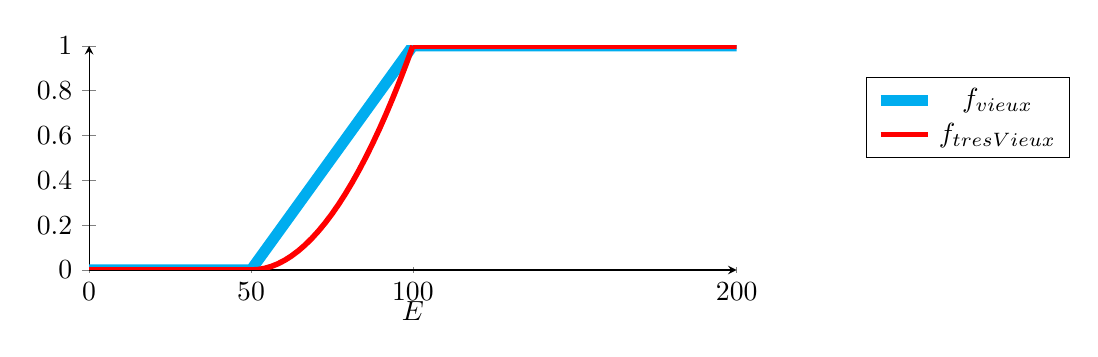
\begin{tikzpicture}
	\begin{axis}[
		xmax=200,
		ymin=0,
		ymax=1,
		xlabel={$E$},
		axis x line=bottom,
		axis y line=left,
		xscale=1.2,
		yscale=0.5,
		xtick=data,
		legend entries={$f_{vieux}$,$f_{tresVieux}$},
		legend style={at={(1,1)},anchor=south west}]
		
			\addplot+[mark=none,line width= 4,cyan] coordinates{(0,0)(50,0)(100,1)(200,1)};
			\addplot+[mark=none,line width= 2,red] coordinates{(0,0)(50,0)};
			\addplot+[domain=50:100,mark=none,line width= 2,red] {1/2500*x^2-1/25*x+1};
			\addplot+[mark=none,line width= 2,red] coordinates{(100,1)(200,1)};
			
	\end{axis}	
\end{tikzpicture} 
